\documentclass[english, 11pt, a4paper]{article}
\usepackage{amsmath, amssymb,amsthm}
\usepackage{setspace, natbib}
\usepackage{bm}
\usepackage{threeparttable}
\usepackage{graphicx}
\usepackage{booktabs}
\usepackage{dcolumn}
\usepackage{tabu}
\usepackage{longtable}
\usepackage{float}
\usepackage{caption}
\usepackage{subcaption}
\usepackage[procnames]{listings}
\usepackage{color}
\setlength{\textwidth}{15.5cm} \setlength{\textheight}{22cm}\setlength{\oddsidemargin}{-0.5mm}
\setlength{\parskip}{1ex plus0.5ex minus0.5ex}\setlength{\parindent}{0mm}
\DeclareMathOperator\erfc{erfc}
\usepackage{babel}


\definecolor{keywords}{RGB}{255,0,90}
\definecolor{comments}{RGB}{0,0,113}
\definecolor{red}{RGB}{160,0,0}
\definecolor{green}{RGB}{0,150,0}
 
\lstset{language=Python, 
        basicstyle=\ttfamily\small, 
        keywordstyle=\color{keywords},
        commentstyle=\color{comments},
        stringstyle=\color{red},
        showstringspaces=false,
        identifierstyle=\color{green},
        procnamekeys={def,class}}


\renewcommand{\bibfont}{\footnotesize}
\setlength{\bibsep}{1pt}

\begin{document}

\baselineskip18pt


\title{Order Book Analysis}

\author{Artagan Malsagov}

\date{\today}


\maketitle


%\section{Introduction}

\section{Data Description}

The data consist of 5 levels of both sides of the order book, for 5 different days.
Each days spans roughly 10 hours worth of data (36 billion micros, see table below)

\begin{table}[H]
    \centering
    \begin{tabular}{lrr}
    \toprule
    date & min timestamp & max timestamp \\
    \midrule
    20190610 & 0 & 36000000000\\
    20190611 & 0 & 36000000000 \\
    20190612 & 0 & 36000000000 \\
    20190613 & 0 & 36000000000 \\
    20190614 & 0 & 35999621354 \\
    \bottomrule
    \end{tabular}
\end{table}

\subsection{Data resampling}
The order book is of the form below:

\begin{table}[H]
    \centering
    \begin{tabular}{crrrr}
    \toprule
    timestamp & bp0 & bq0 & ap0 & aq0 \\
    \midrule
    110 & 10045& 62 & 10055 & 98 \\
    175 & 10065& 46 & 10075 & 42 \\
    220 & 10075& 9 & 10080 & 25 \\
    \bottomrule
    \end{tabular}
\end{table}

where timestamp is in microseconds. Given the 


First a simple plot of the data. The simple mid price is considered:
\begin{equation}
    P_{mid} = \frac{bp0 + ap0}{2}
\end{equation}

Also the inverse weighted mid price is calculated:

\begin{equation}
    P_{mid} = \frac{bp0\times aq0 + ap0 \times bq0}{bq0 + aq0}
\end{equation}

 \begin{figure}[H] 
	\centering
	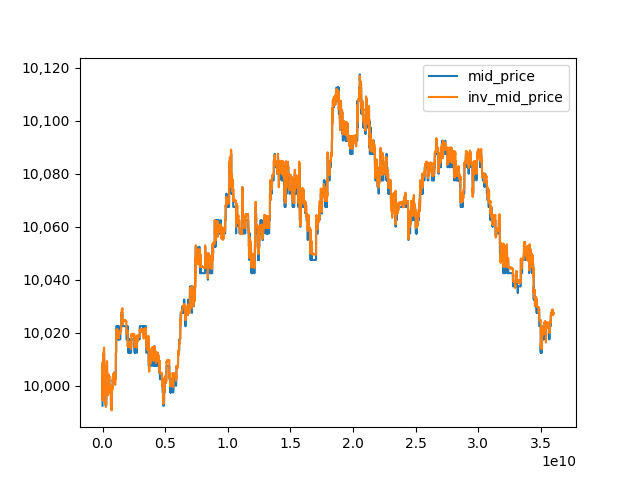
\includegraphics[width=0.90\textwidth]{../data/figures/plot_mid_price_inv_mid_price.png}
	\caption{}
	\label{fig1}
\end{figure}



\section{Model Selection}

\section{Results}

%%\section{Conclusion}       

\bibliographystyle{plain}
%\bibliography{report_sci_comp_3}

\end{document}
